\documentclass[11pt,a4paper]{article}
\usepackage[margin=26mm,headheight=15pt]{geometry}
\usepackage[T1]{fontenc}
\usepackage[utf8]{inputenc}
\usepackage{lmodern,microtype}
\usepackage{amsmath,amssymb,amsthm,mathtools}
\usepackage{booktabs,array,longtable,enumitem}
\usepackage{xcolor,graphicx,tikz,listings,fancyhdr}
\usetikzlibrary{arrows.meta,positioning}
\usepackage[hidelinks]{hyperref}
\usepackage{xurl}
\hypersetup{pdftitle={Ordered Pivot Interfaces: Optimal Positive Handle Cancellation at Bounded Incidence Width},pdfauthor={Research continuation prepared with ChatGPT for the ProveIt project}}
\pagestyle{fancy}\fancyhf{}
\fancyhead[L]{\small Ordered pivot interfaces}
\fancyhead[R]{\small ProveIt research continuation}
\fancyfoot[C]{\thepage}
\renewcommand{\headrulewidth}{0.3pt}
\setlength{\parskip}{4pt}
\setlength{\parindent}{1em}
\setlist{itemsep=2pt,topsep=5pt,leftmargin=*}
\lstset{basicstyle=\ttfamily\small,columns=fullflexible,breaklines=true,frame=single,framerule=0.25pt,xleftmargin=4pt,xrightmargin=4pt,aboveskip=8pt,belowskip=8pt}
\newtheorem{theorem}{Theorem}[section]
\newtheorem{lemma}[theorem]{Lemma}
\newtheorem{proposition}[theorem]{Proposition}
\newtheorem{corollary}[theorem]{Corollary}
\theoremstyle{definition}
\newtheorem{definition}[theorem]{Definition}
\newtheorem{example}[theorem]{Example}
\theoremstyle{remark}
\newtheorem{remark}[theorem]{Remark}
\newcommand{\supp}{\operatorname{supp}}
\newcommand{\OPT}{\operatorname{OPT}}
\newcommand{\wt}{\operatorname{wt}}
\newcommand{\tw}{\operatorname{tw}}
\newcommand{\code}[1]{\nolinkurl{#1}}
\newcommand{\Z}{\mathbb Z}
\newcommand{\N}{\mathbb N}
\newcommand{\mi}{-\infty}
\newcommand{\calS}{\mathcal S}
\newcommand{\calD}{\mathcal D}

\newcommand{\EnumSeven}{243.3}
\newcommand{\DPSeven}{0.673}
\newcommand{\RatioSeven}{361}
\newcommand{\EnumOne}{0.007}
\newcommand{\DPOne}{0.100}
\newcommand{\HugeMillis}{13.7}
\newcommand{\HugeBytes}{895,547}

\begin{document}
\begin{titlepage}
\thispagestyle{empty}
\vspace*{13mm}
{\large\sffamily PROVEIT\quad /\quad UNKNOT RECOGNITION\par}
\vspace{17mm}
{\LARGE\bfseries Ordered Pivot Interfaces\par}
\vspace{5mm}
{\Large Optimal positive handle cancellation\\at bounded incidence width\par}
\vspace{13mm}
{\large A mathematical and computational research continuation\par}
\vspace{5mm}
Prepared with ChatGPT for Vladimir Reshetnikov's ProveIt project\\
12 October 2026
\vspace{14mm}
\begin{abstract}
The existing positive-cancellation calculus can decide whether every active
row disappears by private-column peeling. Selecting the best residual set is
more difficult. We identify its weighted optimization problem with
unit-restricted uniquely restricted matching in a bipartite incidence graph
and prove an exact algorithm with running time
$\operatorname{poly}(N,B)\,2^{O(w\log(w+2))}$, given a width-$w$ tree
decomposition. A bag stores only a total order and one matching-status bit
per vertex. An order-amalgamation lemma replaces a quadratic-size
reachability relation and supplies the join proof.

We extend the ordered states to exact max-plus interfaces for repeat-safe
path templates. Binary repetition is handled in time polynomial in the
encoded repetition length, with independently checked full-table
optimality certificates. A connected family of incidence treewidth two has
full row rank, a unit maximal minor, and an optimal deferred weight growing
linearly with the number of tiles. Thus low-width optimization is useful
without implying small residual cores.

The release includes proofs, a standard-library implementation, independent
plan and transfer checkers, 52 unit tests, exhaustive comparisons on 36,901
matrices, and paired component measurements. It does not supply a general
quasi-polynomial unknot recognizer, authenticate new geometric sources, or
claim an end-to-end knot speedup.
\end{abstract}
\vfill
\noindent\textbf{Provenance.} Targeted source inspection against ProveIt revision\\
\code{ac9c845a5c507c5d7a17d45b2d8de84fc046d455}.\\[3pt]
\textbf{Status.} Mathematical proofs and executable research code; not a
proof-assistant formalization or an independently refereed publication.
\end{titlepage}
\begingroup
\fontsize{9}{10.4}\selectfont
\setlength{\parskip}{0pt}
\tableofcontents
\endgroup
\newpage

\section{Research objective and exact scope}
\label{sec:scope}

\subsection{Where this work enters the recognition pipeline}
The immediate input is an unsigned occurrence matrix reconstructed from a
geometric handle core. Rows represent two-handles; columns represent
one-handle cocores after the selected earlier reductions. A unit entry can
license a geometric cancellation when the surrounding source charts and
attaching-curve data satisfy the native checker's hypotheses. The inspected
\code{core_handlebody.py} explicitly excludes arbitrary group
presentations and signed exponent sums as substitutes for that input
\cite{repo-core}.

The repository already has a complete private-column test for eliminating
\emph{all} rows in its positive calculus. Its queue and the accompanying
stopping-set interpretation are existing work, not contributions claimed
here. Report 102 develops optimal row deferral and exact passive-count
transport; report 103 develops source-relative top-handle elimination and
fixed-forest exceptional-row reductions \cite{repo102,repo103}. Our main
change is to parameterize the \emph{optimization} problem by incidence
width, rather than by the number of rows that must be deferred.

The result is relevant when the complete queue stops but a useful partial
geometric reduction is still wanted. It does not replace the cheap queue
on easy inputs. Section~\ref{sec:preprocess} proves that the queue can be
run first without losing an optimal nonnegative-weight solution.

\subsection{The quasi-polynomial target}
Lackenby's 2021 announcement states a quasi-polynomial recognition target
\cite{lackenby-talk}. His July 2026 preprint develops the hierarchy
algorithm, but Section 9 separates iteration counting from the unestimated
cost of individual operations. Its iteration estimate is $L(g+1)^L$, in
terms of hierarchy length and pattern complexity \cite{lackenby2026}.
The present contribution concerns one possible reduction primitive, not the
complete hierarchy search.

For the explicit matrix problem, our width bound gives a quasi-polynomial
algorithm whenever
\begin{equation}
 w\log(w+2)=O((\log N)^2).
 \label{eq:widthqp}
\end{equation}
Here $N$ is the relevant encoded instance/decomposition size, not
necessarily the crossing number of the original diagram. A reduction
producing such instances from every knot diagram, with bounded total
hierarchy cost, has not been proved here.

\subsection{Contribution and attribution ledger}
\begin{center}\small
\begin{tabular}{p{0.25\textwidth}p{0.66\textwidth}}
\toprule
Item & Status in this article \\
\midrule
Private peeling and stopping sets & Prior ProveIt work; proved again to make the optimization reduction self-contained. \\
Uniquely restricted matching & Classical notion and alternating-cycle characterization; the matrix connection is not new \cite{golumbic2001}. \\
Ordered boundary algorithm & A proved weighted, allowed-unit bipartite specialization with $2^{O(w\log(w+2))}$ dependence, including joins and witnesses. \\
Repeat-safe interfaces & Exact continuation tables, contextual substitution, binary powers, and complete table replay. Max-plus powering itself is elementary; the contribution is the interface contract for this calculus. \\
Connected obstruction family & Explicit treewidth-two, full-row-rank, unit-minor family with exactly computable linear optimal deferral. \\
Geometric integration & A source-aware contract and an additive occurrence adapter, not a production patch or a new topology verifier. \\
\bottomrule
\end{tabular}
\end{center}

Chaudhary, Sau and Zehavi give a deterministic treewidth algorithm for
uniquely restricted matching on general graphs with a quadratic-width
exponent, and ask about improving that dependence \cite{csz2025}.
The bipartite orientation used below gives the smaller exponent for the
subclass needed here, including weights and prohibited unit pivots. It
\emph{does not solve their general-graph question}. The literature search
and targeted source review do not establish an exhaustive priority claim
for every special case of our algorithm.

\section{Positive cancellation, stopping sets, and deferral}
\label{sec:positive}

\subsection{The abstract calculus}
Let $H=(H_{ij})$ be an $m\times n$ matrix over $\Z_{\geq0}$, and let
$c_i\in\Z_{\geq0}$ be a cost for leaving row $i$ unresolved. Empty row or
column sets are permitted. Rows retain their original labels throughout
all operations.

\begin{definition}[Positive unit pivot]
A pivot at $(r,j)$ requires $H_{rj}=1$. It removes row $r$ and column $j$,
and changes the remaining entries to
\begin{equation}
 H'_{ik}=H_{ik}+H_{ij}H_{rk}\qquad (i\ne r,\ k\ne j).
 \label{eq:positive}
\end{equation}
The weight earned is $c_r$. No subtraction, cancellation of opposite
orientations, arbitrary row operation, or free word reduction is allowed.
\end{definition}

A set $S$ of rows is \emph{privately peelable} if one can order its rows
$r_1,\ldots,r_t$ and choose distinct columns $j_1,\ldots,j_t$ such that
\begin{equation}
 H_{r_a j_a}=1,\qquad
 H_{r_b j_a}=0\quad\text{whenever }b>a.
 \label{eq:private}
\end{equation}
Thus column $j_a$ is private among the as-yet-unpeeled rows of $S$.
Rows outside $S$ are passive: they may meet the pivot cocore and are
transported by~\eqref{eq:positive}. They are \emph{not} deleted.

Define
\[
 \OPT(H,c)=\max\Big\{\sum_{i\in S}c_i:S\text{ is privately peelable}\Big\},
 \qquad
 \delta(H,c)=\sum_{i=1}^m c_i-\OPT(H,c).
\]
For unit costs, $\delta$ is the least number of deferred rows. Zero-cost
rows are still real rows, even if an optimum chooses to defer them.

\subsection{Why positive fill does not improve the optimum}
\begin{definition}[Stopping set]
A nonempty set $X$ of rows is stopping if, for every column $j$,
\[
 s_j(X):=\sum_{i\in X} H_{ij}\quad\text{belongs to }\{0,2,3,\ldots\}.
\]
\end{definition}

\begin{lemma}[Stopping-set persistence]
\label{lem:persistence}
Suppose $X$ is stopping and a positive unit pivot removes row $r$ and
column $j$. If $r\notin X$, the same set $X$ is stopping afterward. If
$r\in X$, then $X\setminus\{r\}$ is nonempty and stopping afterward.
\end{lemma}
\begin{proof}
If $r\notin X$, then for each surviving column $k$,
\[
 s'_k(X)=s_k(X)+s_j(X)H_{rk}.
\]
Both summands are nonnegative; a positive second summand is at least two.
Thus a new sum of one cannot occur.

If $r\in X$, then $H_{rj}=1$ and $s_j(X)\ne1$, so
$s_j(X\setminus\{r\})\geq1$. In particular $X\setminus\{r\}$ is
nonempty. Put $t=s_j(X\setminus\{r\})$. For a surviving column $k$,
\[
 s'_k(X\setminus\{r\})
 =s_k(X)+(t-1)H_{rk}.
\]
When $s_k(X)\geq2$, the result is at least two. When $s_k(X)=0$,
nonnegativity implies $H_{rk}=0$, so the result is zero.
\end{proof}

\begin{theorem}[Exact positive/private equivalence]
\label{thm:positive-private}
For a prescribed row set $S$, the following are equivalent.
\begin{enumerate}[label=(\roman*)]
\item A sequence of positive unit pivots removes exactly the rows of $S$.
\item The original submatrix on $S$ has no stopping subset.
\item $S$ is privately peelable.
\end{enumerate}
Consequently $\OPT(H,c)$ is the maximum weight removable by
\emph{any} positive unit-pivot sequence, including fill-producing ones.
\end{theorem}
\begin{proof}
If a stopping set $X\subseteq S$ existed, repeatedly apply
Lemma~\ref{lem:persistence} along a sequence removing $S$. Its surviving
part remains nonempty, which contradicts removal of every row of $S$.
This proves (i)$\Rightarrow$(ii).

Under (ii), any nonempty remaining subset $Y\subseteq S$ has a column
with $s_j(Y)=1$. Its unique nonzero entry is one. Peel that row and repeat;
every smaller subset still contains no stopping set. The selected column
has no entry on any other remaining active row, so it cannot be needed as
a later nonzero pivot column. This constructs~\eqref{eq:private}.

Finally, perform the private schedule in the full matrix. At each step
all other active rows have zero in the pivot column. Formula~\eqref{eq:positive}
therefore leaves their other entries unchanged. Passive rows may change,
but they do not alter active-row privacy. All selected pivots remain unit,
so the schedule is legal and removes exactly $S$.
\end{proof}

This theorem concerns the positive model. It does not assert that arbitrary
geometric handle slides or signed algebraic simplifications have the same
optimum. With an externally restricted set of allowed pivot edges, our
algorithm optimizes private schedules using those edges. Unless separately
proved, Theorem~\ref{thm:positive-private} should not be read as a
completeness theorem for every differently restricted fill-producing
calculus.

\begin{proposition}[Capping and an integral rank bound]
\label{prop:capping}
Replacing every entry $x$ by $\min(2,x)$ preserves private peelability and
$\delta(H,c)$. A privately peelable set of $t$ rows determines a $t\times t$
minor with determinant one after ordering its rows and pivot columns.
In particular, for unit costs,
\[
 \delta(H,\mathbf1)\geq m-\operatorname{rank}_{\mathbb Q}H,
 \qquad
 \delta(H,\mathbf1)\geq m-n.
\]
\end{proposition}
\begin{proof}
The private test uses only the distinctions zero, one, and larger than
one. Its selected submatrix satisfies~\eqref{eq:private}, so is upper
triangular with all diagonal entries one. It has rank $t$ and determinant
one. The two inequalities follow from $t\leq\operatorname{rank}H$ and
$t\leq n$.
\end{proof}

Capping is only an optimization invariant. It is not an exact transport
representation for passive multiplicities or embedded attaching curves.
Section~\ref{sec:barrier} shows that even a unit maximal minor need not make
the deferral small.

\section{The bipartite matching formulation}
\label{sec:matching}

Let $G_H$ have row vertices $R=\{r_1,\ldots,r_m\}$, column vertices
$C=\{q_1,\ldots,q_n\}$, and edge $r_iq_j$ exactly when $H_{ij}>0$.
This is the \emph{support incidence graph}. It is not the graph obtained
by making all rows meeting one column into a clique.

Let $U$ be any subset of the edges with $H_{ij}=1$. A matching is
\emph{unit-allowed} if it is contained in $U$. By default every unit edge
is allowed. Entries larger than one remain support edges, although they
cannot be matching edges.

\begin{definition}[Matching orientation]
For a unit-allowed matching $M$, orient every edge not in $M$ from its row
to its column, and every edge in $M$ from its column to its row. Denote the
resulting directed graph by $D_M$.
\end{definition}

\begin{lemma}[Bipartite directed-cycle characterization]
\label{lem:directed}
$D_M$ is acyclic if and only if $M$ has no alternating cycle. Equivalently,
$M$ is the unique perfect matching of the subgraph induced by its matched
vertices.
\end{lemma}
\begin{proof}
At a row vertex, the only possible incoming edge is its matching edge;
at a column vertex, the only possible outgoing edge is its matching edge.
A directed cycle therefore alternates matching and nonmatching edges.
Conversely, either traversal of an alternating cycle that begins with a
nonmatching row-to-column edge follows the orientation all the way around.

If a second perfect matching on the same vertices existed, its symmetric
difference with $M$ would contain an alternating cycle. Flipping the two
classes of edges of such a cycle produces a second perfect matching.
\end{proof}

\begin{theorem}[Triangular matching equivalence]
\label{thm:matching}
A row set $S$ has a private schedule using allowed unit pivots if and only
if it is the set of matched row vertices of an allowed matching $M$ for
which $D_M$ is acyclic. Hence
\begin{equation}
 \OPT_U(H,c)=\max_{\substack{M\subseteq U\text{ matching}\\D_M\text{ acyclic}}}
             \sum_{r_iq_j\in M} c_i.
 \label{eq:matching-opt}
\end{equation}
For unrestricted unit pivots this is the positive optimum of
Theorem~\ref{thm:positive-private}.
\end{theorem}
\begin{proof}
A private schedule supplies distinct pivot edges. Among matched rows,
any other row $r_b$ touching the pivot column of $r_a$ must have $b<a$.
In a directed cycle, every two-edge segment has the form
$r_b\to q_{j_a}\to r_a$, and therefore strictly increases the schedule
index. This is impossible around a cycle. Unmatched rows cannot lie on a
directed cycle because they have no incoming edges; unmatched columns
have no outgoing edges.

Conversely, choose a topological order of $D_M$ and list matched rows in
that order. If another matched row $r_b$ meets the pivot column of $r_a$,
then the directed path $r_b\to q_{j_a}\to r_a$ puts $r_b$ earlier. Thus
the pivot column of each next row is private among later matched rows.
\end{proof}

The optimization of uniquely restricted matchings is already difficult
on bipartite graphs \cite{golumbic2001}. The incidence-width restriction
below is therefore substantive. It is not a reformulation that makes the
unrestricted optimization polynomial.

\subsection{A compact independent witness}
A feasible result can be recorded simply as the list of matched unit
edges, together with the deferred row inventory and objective. The checker
first tests distinct endpoints and allowed unit counts. It then builds the
directed dependency graph on matched rows:
\begin{equation}
 r_b\longrightarrow r_a
 \quad\Longleftrightarrow\quad
 b\ne a\text{ and }H_{b,j_a}>0.
 \label{eq:rowdependency}
\end{equation}
A topological sort yields a private schedule; a directed cycle rejects the
witness. This checker uses no tree-decomposition states.

A sparse implementation of~\eqref{eq:rowdependency} uses at most one
inspection of each relevant occurrence because each pivot column has one
owner. The supplied reference checker uses a simpler dense loop over
matched row pairs. Neither this feasible witness nor its topological sort
certifies \emph{optimality}. Optimality follows from the complete DP or,
for the repeated-template component, from the full-table proof in
Section~\ref{sec:proofdag}.

\section{Ordered boundary states and the width theorem}
\label{sec:width}

\subsection{A gluing lemma for total orders}
\begin{lemma}[Order amalgamation]
\label{lem:amalgamation}
Let $V_1\cap V_2=B$, and let $<_1,<_2$ be total orders on $V_1,V_2$
whose restrictions to $B$ agree. There is a total order on $V_1\cup V_2$
restricting to each given order.
\end{lemma}
\begin{proof}
List $B$ as $b_1<\cdots<b_k$. Each order separates its other vertices
into $k+1$ ordered lists: before $b_1$, between consecutive $b_i$, and
after $b_k$. For every gap, merge its two lists in any way preserving their
individual orders. Insert the common $b_i$ between these merged lists.
For $B=\varnothing$, merge the two entire lists.
\end{proof}

The lemma has a useful directed version. If each side is acyclic and has
a topological order restricting to the same total order on $B$, the union
is acyclic: amalgamate the two topological orders. Notice that it is not
enough merely to remember that each side is acyclic. A common compatible
boundary order is the certificate that rules out a cycle assembled from
paths on opposite sides.

\subsection{Decomposition and states}
Assume a tree decomposition of $G_H$ is supplied and validated: every
vertex occurs, every edge is covered by a bag, and the bags containing
any fixed vertex form a connected subtree. Let the maximum bag size be
$b=w+1$. Use an empty root and empty leaves, vertex-introduction,
vertex-forgetting, edge-introduction, and binary join operations. Each
support edge is introduced exactly once.

For a bag $B$, a state is
\begin{equation}
 (\pi,\mu),\qquad
 \pi\text{ a total order of }B,\qquad \mu:B\to\{0,1\}.
 \label{eq:state}
\end{equation}
The flag $\mu(v)$ says that $v$ is already matched by an edge introduced
in the processed subproblem. A table entry is the maximum weight of that
partial matching subject to two conditions: its matching orientation is
acyclic, and it has a topological order whose restriction to $B$ is $\pi$.
The table stores an existential extension, not a unique topological order.
An absent entry means infeasibility.

There is no requirement that a forgotten vertex was matched. An unmatched
forgotten row is a deferred row; an unmatched forgotten column is unused.
No mate label is needed: the already-introduced matching edges carry their
own endpoints, and the flag is enough to prevent a second edge using one
of them.

\subsection{Transitions}
The empty leaf has value zero at its unique empty state.

\paragraph{Introduce a vertex $v$.}
Insert $v$ into any of the $|B|+1$ positions of the child order and set
$\mu(v)=0$. No incident processed edge exists yet in this branch. Inserting
$v$ into a specified boundary gap is compatible with an extension of the
old order to all forgotten vertices: place $v$ anywhere in that same gap.

\paragraph{Introduce a support edge $r_iq_j$.}
If $r_i<_\pi q_j$, leave the edge outside the matching. The state and
score are unchanged. If $q_j<_\pi r_i$, this edge must be in the matching:
require $r_iq_j\in U$ and $\mu(r_i)=\mu(q_j)=0$, set both flags to one,
and add $c_i$. These are the only cases. In particular, a nonunit edge
cannot be oriented backward by the algorithm.

\paragraph{Forget a vertex $v$.}
Delete $v$ from the order and from the flags, and maximize over all child
states projecting to the same result. The existence of an extending total
order is preserved.

\paragraph{Join two subproblems.}
Only equal boundary orders can be joined. The two flag sets must be
disjoint, and the new flag set is their union. Add the two scores and take
the maximum. Edges belong to only one subproblem, so no reward is counted
twice.

\begin{theorem}[Correctness of the ordered-interface DP]
\label{thm:dp}
The transitions above compute~\eqref{eq:matching-opt} exactly, and can
return an allowed private schedule attaining the value.
\end{theorem}
\begin{proof}
We prove the table invariant by induction on the decomposition.
Vertex and edge introduction are sound by their definitions: every
introduced directed edge agrees with the stored boundary order, and the
flags enforce a matching. Conversely, any feasible extension has the
specified order of its two endpoints, so is represented by exactly the
applicable edge case. Forgetting is existential projection.

At a join, the interiors of the two subproblems are disjoint by the
running-intersection property. Their common vertices are exactly the
boundary vertices that both use. If flags are disjoint, the union is a
matching. Select topological orders witnessing the two equal boundary
orders. Lemma~\ref{lem:amalgamation} gives a topological order of the union,
so no directed cycle is introduced. This proves soundness at the only
nonlocal operation.

For completeness, take any feasible matching on the union and a global
topological order. Restrict both to the two child subproblems. Their
boundary orders agree, their flag sets are disjoint, and their rewards
add. Thus the DP considers this solution. Taking maxima preserves the
best one. At the empty root there are no remaining boundary conditions,
so the value is the global optimum. Store maximizing predecessor choices
and selected edges; Theorem~\ref{thm:matching} converts the result to a
private schedule.
\end{proof}

\subsection{State and bit complexity}
Let $s$ count the elementary decomposition operations, including edge
introductions, and put
\[
 S_b=b!\,2^b,\qquad
 \Lambda=1+\left\lceil\log_2\left(1+\sum_i c_i\right)\right\rceil.
\]
Pointer and vertex-label bit lengths must also be included in the encoded
cost. Let $B_0$ denote the total input bit length before decomposition
normalization.

\begin{theorem}[Incidence-width optimization bound]
\label{thm:widthbound}
Given a validated width-$w$ decomposition, weighted allowed-unit private
cancellation can be optimized in
\begin{equation}
 O\!\left(s\,\operatorname{poly}(b,\Lambda,\log(s+2))\,b!\,3^b+B_0^{O(1)}\right)
 =\operatorname{poly}(N,B_0)\,2^{O(w\log(w+2))}
 \label{eq:time}
\end{equation}
bit time, with $O(sS_b)$ table/witness records of polynomial bit size.
For unrestricted unit pivots this optimizes all positive unit-pivot
sequences. No bound on the optimal deferred weight is assumed.
\end{theorem}
\begin{proof}
A bag of size at most $b$ has at most $b!2^b$ states. Introductions and
projections inspect these states with polynomial work per state. For a
fixed order at a join, each boundary vertex is matched on the left, on the
right, or on neither side. There are $3^b$ disjoint flag pairs. Enumerating
a left flag set and the submasks of its complement realizes this count;
there is no need to inspect all $4^b$ pairs. Each finite score lies between
zero and $\sum_i c_i$, so score arithmetic uses at most $\Lambda$ bits.
The input counts are only tested for zero and one after being read; their
magnitudes do not enter the table dimensions. Decomposition validation,
edge assignment, and normalization have polynomial encoded cost.

Maximizing predecessor pointers and chosen matching edges can be retained
with the tables. A persistent witness representation shares predecessors;
it does not copy a complete matching into every state. Stirling's bound
$\log_2(b!)=O(b\log(b+1))$ gives the stated exponential dependence.
\end{proof}

For the explicit leading bound, permutations and masks can be ranked into
indexed tables, or deterministic search-tree lookup costs can be included
in the polynomial factor. The Python prototype uses dictionaries; even
worst-case lookup overhead does not change the coarser
$2^{O(w\log(w+2))}$ bound.

The supplied Python implementation includes a deterministic minimum-fill
\emph{heuristic} for constructing a decomposition. It validates the result,
but does not certify that its width is minimum or close to minimum. Its
preprocessing is polynomial and can be a significant practical cost. A
supplied better decomposition may be used directly. A state limit is an
inconclusive resource outcome, not a negative optimization or topological
certificate. In the reference implementation that limit is checked after
a transition table is constructed, so it is not a strict allocation cap.

\begin{corollary}[Restricted quasi-polynomial optimization]
\label{cor:qp}
If the encoded input and supplied decomposition have size $N^{O(1)}$, and
$w\log(w+2)=O((\log N)^2)$, then optimal positive deferral is computable in
$N^{O(\log N)}$ time. The stronger condition $w=O(\log N)$ gives
$N^{O(\log\log(N+2))}$ time, up to polynomial input-bit factors.
\end{corollary}
\begin{proof}
Substitute the width conditions into~\eqref{eq:time}. For example,
$w=O((\log N)^2/\log\log(N+3))$ is sufficient for the first condition.
\end{proof}

This is a restricted \emph{optimization} theorem. It supplies neither a
small optimal residual nor a sequence of admissible hierarchy surfaces.

\section{Exact preprocessing and source-preserving residuals}
\label{sec:preprocess}

\begin{lemma}[A private leaf is safe to take first]
\label{lem:forced}
Suppose column $j$ has total incidence one in the entire current matrix,
with its unit entry in row $r$. Let $H^-$ be obtained by removing row $r$
and column $j$. For nonnegative row weights,
\[
 \OPT(H,c)=c_r+\OPT(H^-,c|_{R\setminus\{r\}}).
\]
\end{lemma}
\begin{proof}
Any private schedule in $H^-$ can be preceded by $(r,j)$; this pivot
changes no other row because its column is private in the full matrix.
This gives the lower bound. For the reverse bound, take a privately
peelable set $S$ in $H$. If $r\notin S$, column $j$ is identically zero
on $S$, so its deletion does not affect that schedule. If $r\in S$,
hereditary peelability gives a private schedule for $S\setminus\{r\}$,
and its nonzero pivot columns cannot include $j$. In either case its
reward is at most $c_r+\OPT(H^-,c)$, using $c_r\geq0$.
\end{proof}

\begin{theorem}[Peel first, optimize only the stopping residual]
\label{thm:prepass}
Run the existing complete private-column queue until it stops. Let $P$ be
the removed rows and let $H_C$ be the remaining occurrence matrix, with
isolated optimization columns optionally omitted. Then
\[
 \OPT(H,c)=\sum_{r\in P}c_r+\OPT(H_C,c|_C),
 \qquad \delta(H,c)=\delta(H_C,c|_C).
\]
Restricting a supplied tree decomposition to the residual incidence graph
does not increase its width.
\end{theorem}
\begin{proof}
Iterate Lemma~\ref{lem:forced}. Isolated columns cannot supply a pivot and
can be omitted from an optimization instance. Intersecting every bag with
the surviving vertex set preserves edge coverage and running intersection;
empty bags can be retained or removed conventionally.
\end{proof}

The implementation \code{peel_then_optimize} uses the queue before the DP.
It preserves source row and column labels in the returned plan, and
replays that plan against the original matrix. On a complete private-peel
instance it creates no DP states. This wrapper currently requires
unrestricted unit pivots, rather than silently assuming the same forcing
proof for arbitrary pivot restrictions.

An omitted optimization column is \emph{not} a removed geometric
one-handle. A deferred row that becomes numerically zero is \emph{not}
a removed geometric two-handle. The output is a cancellation schedule plus
an unresolved inventory; geometry retains everything not explicitly
cancelled by an authenticated operation.


\subsection{Strict partial improvement over the inspected minimum-fill rule}
\label{sec:minfill}
The native file keeps a capped minimum-fill producer and comparison rule
\cite{repo-core}. For a unit entry $(r,j)$ it minimizes lexicographically
\[
 ((s_r-1)(t_j-1),\ s_r,\ r,\ j),
 \quad s_r=\sum_k H_{rk},\quad t_j=\sum_i H_{ij},
\]
with each matrix entry capped at two after an update. Its full-completion
property does not make its partial schedule optimal.

\begin{example}[Two greedy cancellations versus three optimal ones]
\label{ex:minfill}
Use zero-based source row and column labels and the matrix
\[
 A=\begin{pmatrix}
 2&0&1&0\\
 0&1&1&0\\
 1&1&0&1\\
 0&1&1&2
 \end{pmatrix}.
\]
The inspected rule first chooses $(1,1)$ and then $(2,0)$. The two
remaining capped rows, on the surviving columns $2,3$, are both $(2,2)$,
so it stops after two cancellations. In contrast, defer row $3$ and use
\[
 (2,3),\quad (1,1),\quad (0,2).
\]
These columns are private among the selected active rows at the time they
are used. Every original full column sum is three, so all four rows form
a stopping set. Thus full cancellation is impossible, and three is the
exact optimum, independently of the DP. Exact passive transport leaves
row $3$ with the single surviving count $A'_{3,0}=10$.
\end{example}

The supplied test checks the heuristic's precise tie-breaking rule, the
optimal private plan, the stopping-set upper bound, and the exact passive
count. It uses a labelled reference transcription, not an import of the
full native file. This is a strict improvement in what can be selected
from the same \emph{abstract} occurrence data, not evidence of a new
accepted geometric source. It is also not a correctness bug in the old
routine: that routine does not promise an optimal partial reduction.

\section{Repeat-safe path templates and exact continuation tables}
\label{sec:templates}

\subsection{The template contract}
A typed boundary consists of finitely many named row/column vertices, with
a nonnegative weight attached to each row name. A path template has an
input boundary, a sequence of operations, and a bijective renaming of its
final live vertices onto an output boundary. Operations introduce a fresh
vertex, introduce a support edge between live row/column endpoints, or
forget a live vertex. Every edge has a positive count and an allowed-unit
flag. Every live bag has size at most $b$.

The implemented \emph{repeat-safe} class satisfies all of the following:
vertices are introduced fresh within a copy, each support edge is introduced
once, an edge involves at least one vertex fresh within that copy, and
boundary renaming preserves types and weights when a template is repeated.
No edge may be introduced between two input vertices. These conditions
make repeated copies edge-disjoint except for their specified shared
boundary vertices. A reused input name is an identified vertex, not a
fresh occurrence with an accidentally equal label.

The freshness restriction is sufficient, not necessary. It deliberately
excludes some legal graph grammars rather than infer, without evidence,
that repeated interface-interface entries are distinct or should be added
to one coefficient. A more general authenticated grammar could carry an
explicit once-only edge ownership rule.

\subsection{The exact transfer matrix}
For a boundary $B$, use the ordered states $\calS(B)$
of~\eqref{eq:state}. The incoming flags now mean that those boundary
vertices are already matched \emph{before} the template begins.
For a template $P$, define
\[
 T_P(s,t)\in\Z_{\geq0}\cup\{\mi\}
\]
to be the largest additional matched-row weight achievable through the
template from state $s$ to state $t$. A flag initially equal to one cannot
be matched again. A freshly introduced row earns its weight only if one
of its incident edges is chosen; a persistent input row can earn its
weight here only when it was not already matched.

Each input state can be propagated by the vertex/edge/forget transitions
of Section~\ref{sec:width}. Output labels are then renamed simultaneously.
The finite table contains every order and flag state, including states
unreachable from an empty exterior but relevant in a different context.

\begin{theorem}[Exact composition and contextual replacement]
\label{thm:composition}
Suppose the output boundary of $P$ agrees with the input boundary of $Q$,
and the templates satisfy the ownership and freshness conditions. Then
\begin{equation}
 T_{PQ}(s,u)=\max_{t\in\calS(B)}\bigl(T_P(s,t)+T_Q(t,u)\bigr),
 \label{eq:maxplus}
\end{equation}
with $\mi+x=\mi$. Consequently, equal transfer tables are interchangeable
in every compatible typed prefix/suffix context for matched-weight
optimization. For deferred weight, also retain the total weight of fresh
rows introduced by each template.
\end{theorem}
\begin{proof}
A feasible schedule through $PQ$ has a state $t$ at the common boundary.
Its matching flags record exactly which common vertices have already
been used, so its restrictions are feasible through the two factors and
its rewards add. This gives the upper bound in~\eqref{eq:maxplus}.

Conversely choose maximizing transitions through $P$ and $Q$ at a common
state $t$. Matching flags prevent a double use of a common vertex.
Compatible boundary orders admit a common topological extension by
Lemma~\ref{lem:amalgamation}, or equivalently by successively inserting the
forgotten vertices into their boundary gaps. The two parts therefore give
an acyclic matching on the concatenation. Edge ownership prevents
multiplicity or reward duplication. This proves the lower bound. Repeated
application gives contextual replacement. Deferred weight is total source
row weight minus matched weight, so that total must be carried separately.
\end{proof}

This is a max-plus, not a counting, construction. Several states can
witness different topological orders of the same matching. That is harmless
for maximization but would overcount matchings under naive replacement of
max by addition.

\subsection{Why one scalar is insufficient}
\begin{example}[Two fragments with equal isolated optimum]
\label{ex:scalar}
Take a one-column input port $p$ and one-column output port $q$.
A path fragment has one unit-weight row meeting both ports once. A defect
fragment has two unit-weight rows, both meeting $p$ and a private internal
column $u$ once, and meeting $q$ once and twice respectively. With state
indices $0,1$ denoting whether the single port is already matched,
\[
 T_{\rm path}=\begin{pmatrix}1&1\\0&1\end{pmatrix},\qquad
 T_{\rm defect}=\begin{pmatrix}1&1\\1&1\end{pmatrix}.
\]
Their isolated optimum is one. Prepend a row of weight three meeting only
$p$, and append a row of weight three meeting only $q$. For the path the
optimum is six: both port columns are needed by the two heavy rows. For
the defect the internal column permits one extra row, so the optimum is
seven. The difference is the $(1,0)$ transition. An isolated scalar
optimum does not preserve continuation behavior.
\end{example}

\subsection{Binary powers and encoded complexity}
\begin{theorem}[Binary repetition]
\label{thm:powers}
Let $P$ be a repeat-safe template with equal typed input/output boundaries
and maximum live bag size $b$. Let $W\geq0$ be given in binary. Its full
power transfer table can be computed with at most
$O(\log(W+1))$ max-plus matrix products after compiling $P$. With
$S\leq b!2^b$ interface states, a direct implementation uses
\begin{equation}
 O\!\left(S^3\log(W+1)\,
     \operatorname{poly}(B+\log(W+1))
     +|P|\operatorname{poly}(b)S^2\operatorname{poly}(B)\right)
 \label{eq:powerbound}
\end{equation}
bit time. In particular it is
$\operatorname{poly}(|P|,B,\log(W+1))2^{O(b\log(b+1))}$.
\end{theorem}
\begin{proof}
The identity transfer has zeros on its diagonal and $\mi$ elsewhere.
Equation~\eqref{eq:maxplus} is associative. Binary exponentiation therefore
computes $T_P^W$ by repeated squaring and multiplication. Each product
uses at most $S^3$ score additions/comparisons. A finite score is bounded
by the initial boundary row weight plus $W$ times the fresh-row weight of
one template. Its bit length is $O(B+\log(W+1))$. Compiling the template
once for each input state gives the displayed conservative second term.
\end{proof}

The bit-cost statement counts a supplied binary exponent, not the number
of expanded tiles. For a concatenation-and-power grammar, use its full
encoded derivation DAG and the bit length of the expansion count; nested
binary powers can increase that count, and their lengths must be accounted
for rather than treated as unit-cost integers.

For a completely closed query, input boundary vertices start unmatched.
Maximize the final table over all compatible initial orders with zero
flags and over every final state. The unmatched input vertices and every
freshly introduced row constitute the actual row inventory. Persistent
names are counted only once. Producing a flat list of all expanded
cancellations can require $\Omega(W)$ output, which is not included in the
compressed query bound.

\section{Independently checkable power optimality}
\label{sec:proofdag}

A feasible elimination plan certifies a lower bound on matched weight,
not an upper bound. The power component supplies a stronger certificate:
a DAG of complete transfer tables, with explicit identity, template and
product nodes. Each node also stores the number of template copies it
represents. Product children must be earlier nodes, and their lengths must
sum to the parent's length.

At a product node $C=A\otimes B$, each finite entry stores one maximizing
intermediate state $k$. The checker verifies the following for every
$(i,j)$:
\begin{equation}
 C_{ij}\geq A_{i\ell}+B_{\ell j}
 \quad\text{for every finite candidate }\ell,
 \qquad
 C_{ij}=A_{ik}+B_{kj}.
 \label{eq:optimalitycheck}
\end{equation}
If $C_{ij}=\mi$, it checks that no finite candidate exists and that no
maximizing witness was supplied. Missing or forged infinities cannot be
used to hide a better solution.

\begin{theorem}[Complete-table certificate soundness]
\label{thm:checker}
If the independent checker accepts a power certificate, every stored
transfer table equals the table of its recorded derivation, the root
represents exactly $W$ copies, and the reported closed optimum and deferred
weight are correct for the abstract template expansion.
\end{theorem}
\begin{proof}
The checker recomputes the template table by an implementation that does
not import the producer. Identity tables are checked entry by entry.
Inductively, inequalities and equality in~\eqref{eq:optimalitycheck} prove
that a product entry is exactly the maximum of all candidates. The absence
of a finite candidate proves an infinite entry. Topologically ordered
references prevent circular justification. Length identities prove the
claimed expansion count. Finally the checker recomputes the closed
boundary maximization and subtracts it from the authenticated abstract row
weight inventory.
\end{proof}

The producer uses positional bit masks; the independent template checker
uses named orders and frozen sets of matched names. The mathematical
recurrences are necessarily the same, but their bookkeeping implementations
are separate. Small instances are additionally checked by explicit graph
expansion and independent row-subset optimization.

The certificate has $O(S^2\log(W+1))$ table entries and intermediate
witnesses. Recording all intermediate scores and lengths can use
$O(S^2\log(W+1)(B+\log(W+1)+\log S))$ bits. This quadratic logarithmic
factor in the worst case is not suppressed by pretending that large
integers are machine words. A more compact arithmetic-circuit format might
reduce redundant length/score storage, but is not required for the claimed
polynomial encoded bound.

An accepting certificate does not authenticate an embedding, surface
normal vector, boundary pattern, or cocore atlas. Those are separate source
objects and are absent from this abstract certificate language.

\section{A connected full-rank obstruction at treewidth two}
\label{sec:barrier}

For $q\geq1$, let $H_q$ have rows $a_i,b_i$ for $1\leq i\leq q$ and
columns $v_0,u_1,v_1,u_2,v_2,\ldots,u_q,v_q$. Its only nonzero entries are
\begin{equation}
\begin{array}{c|ccc}
 &v_{i-1}&u_i&v_i\\\hline
 a_i&1&1&1\\
 b_i&1&1&2
\end{array}
\qquad(1\leq i\leq q).
\label{eq:family}
\end{equation}
Give $a_i,b_i$ weights $\alpha_i,\beta_i\geq0$.

\begin{figure}[ht]
\centering
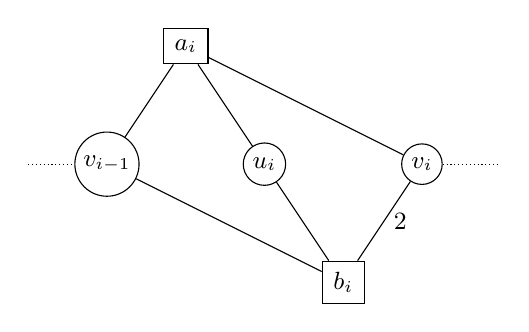
\begin{tikzpicture}[every node/.style={font=\small},x=1cm,y=1cm]
\node[draw,circle,inner sep=2pt] (p) at (0,0) {$v_{i-1}$};
\node[draw,circle,inner sep=2pt] (u) at (2,0) {$u_i$};
\node[draw,circle,inner sep=2pt] (q) at (4,0) {$v_i$};
\node[draw,rectangle,inner sep=4pt] (a) at (1,1.5) {$a_i$};
\node[draw,rectangle,inner sep=4pt] (b) at (3,-1.5) {$b_i$};
\foreach \x in {p,u,q} {\draw (a)--(\x);}
\draw (b)--(p);\draw (b)--(u);\draw (b)--node[right] {$2$}(q);
\draw[densely dotted] (-1,0)--(p);
\draw[densely dotted] (q)--(5,0);
\end{tikzpicture}
\caption{One tile of $H_q$. Unlabelled incidences have count one. Consecutive
tiles share the column $v_i$. The drawing records incidences, not an
embedding or a manifold realization.}
\end{figure}

\begin{theorem}[Low width does not imply small positive residual]
\label{thm:barrier}
The support graph of $H_q$ is connected and has treewidth exactly two.
The matrix has full row rank $2q$ over $\mathbb Q$ and a $2q\times2q$
minor of determinant one. Nevertheless,
\begin{equation}
 \delta(H_q,c)=\sum_{i=1}^q\min(\alpha_i,\beta_i),\qquad
 \OPT(H_q,c)=\sum_{i=1}^q\max(\alpha_i,\beta_i).
 \label{eq:familyopt}
\end{equation}
In particular $\delta(H_q,\mathbf1)=q$.
\end{theorem}
\begin{proof}
The two rows of tile $i$ have total incidences $2,2,3$ on its three
columns, and zero elsewhere. Thus $\{a_i,b_i\}$ is stopping. By
Theorem~\ref{thm:positive-private}, no removable set can contain both rows.
At least the cheaper row in each pair must be deferred, giving the lower
bound for $\delta$. Choose a maximum-weight row in every pair. Its column
$u_i$ is private among all chosen rows, so all chosen rows can be removed,
attaining the bound.

Each tile has support $K_{2,3}$; consecutive tiles share one column
vertex, which makes the whole graph connected. A path decomposition is
obtained by concatenating the bags
\[
 \{a_i,b_i,v_{i-1}\},\quad
 \{a_i,b_i,u_i\},\quad
 \{a_i,b_i,v_i\}.
\]
All bags have size three. Their running intersections hold at the shared
$v_i$ and at the two rows within each tile. Thus treewidth is at most two.
The graph contains a four-cycle, so it is not a forest; hence its treewidth
is not at most one, proving equality.

Delete column $v_0$ and order remaining columns in pairs $(u_i,v_i)$,
with row pairs $(a_i,b_i)$ in increasing $i$. The resulting square matrix
is block lower triangular, with diagonal blocks
$\left(\begin{smallmatrix}1&1\\1&2\end{smallmatrix}\right)$ of determinant
one. Its determinant is one, so $H_q$ has full row rank.
\end{proof}

The family is not a block-diagonal padding construction. Its graph is
connected, the adjacent tiles share a genuine continuation column, and
both rank and maximal-minor tests fail to detect the large positive
residual. We make no claim here that these matrices occur as the specific
native source cores of a family of knot diagrams. That would require a
separate realization and source-chart proof.

\begin{corollary}[A binary-sized optimal residual]
For constant weights $(\alpha,\beta)$, the repeated tile has a two-state
boundary transfer
\begin{equation}
 T=\begin{pmatrix}
 \max(\alpha,\beta)&\alpha\\
 \max(\alpha,\beta)&\alpha
 \end{pmatrix}.
 \label{eq:defect-transfer}
\end{equation}
For $q=2^k$, its exact optimal deferred weight is
$2^k\min(\alpha,\beta)$ and has an $O(k)$-node power derivation, despite
an exponentially large expanded residual inventory.
\end{corollary}
\begin{proof}
At most one row is matched in each tile. With output flag zero, either
row can use $u_i$, regardless of the input flag. With output flag one,
the only allowed edge to $v_i$ is the unit edge from $a_i$, so the reward
is $\alpha$. All four transitions are feasible with the indicated reward.
The optimum and power bound now follow from
Theorems~\ref{thm:barrier} and~\ref{thm:powers}.
\end{proof}

This separates three questions that should not be conflated: whether an
optimum can be found quickly, whether its residual is small, and whether
a large residual can be represented and subsequently processed without
expansion.

\section{Geometric use and the recognition boundary}
\label{sec:geometry}

\subsection{A conditional geometric lifting statement}
\begin{proposition}[Source-conditional reduction]
\label{prop:geometry}
Suppose a source-authenticated handle presentation exports $H$ as its
unsigned cocore-occurrence matrix, and the native geometric verifier
validates the unit cancellations and transports all surviving attaching
curves and protected boundary data through the selected private schedule.
Then the schedule returned by the optimizer is a valid sequence of those
geometric cancellations, leaving exactly the reported uncancelled
row labels. Among schedules in the abstract positive calculus it minimizes
the assigned nonnegative deferred weight.
\end{proposition}
\begin{proof}
The independent matrix checker proves that each selected active pivot
is unit and private. The assumed source verifier supplies precisely the
geometric legality and transport not contained in that matrix statement.
Composing its accepted moves preserves the source topology in the manner
specified by its contract. The weighted optimality assertion is
Theorem~\ref{thm:dp}, together with
Theorem~\ref{thm:positive-private} for unrestricted pivots.
\end{proof}

The transport hypothesis is not a formality. A passive row can cross a
pivot cocore many times, and its cyclic attaching order, side choices,
framing conventions, and inherited marked intersections are not determined
by an unsigned count. The matrix optimizer is not a replacement for a
private-cocore transport or marked-interface exporter.

\subsection{Recommended insertion point}
Use the already authenticated occurrence rows after the fixed primal/top
forest choices. Run the native complete private queue first. On its
stopping residual, construct and validate an incidence decomposition,
then run the bounded optimizer subject to a local resource budget. Replay
the resulting matched edges independently against the original occurrence
rows, not against a producer-supplied transformed matrix. Pass the schedule
to the existing geometric replay and retain all unresolved two-handles.

The archive's \code{integration/occurrence_adapter.py} is additive research
code. It preserves arbitrary nonnegative source labels and reports
\code{REDUCTION_PLAN} or \code{INCONCLUSIVE}; it never reports
\code{UNKNOT}, \code{KNOTTED}, or a handlebody census. It includes a
size guard on its dense adaptation and an inconclusive state budget.
It has been tested on synthetic source-label fixtures, not applied to a
full ProveIt checkout.

Even when $\delta=0$, a knot verdict requires all the other hypotheses of
its actual terminal pipeline. When $\delta>0$, a nonempty stopping residual
only obstructs completion by this calculus. It is not a non-handlebody
certificate, much less a knottedness certificate.

\subsection{What would be needed for an end-to-end theorem}
For a diagram with $n$ crossings, write $Q(n)$ for the number of core
queries and $C_{\rm other}(n)$ for all discovery, source validation,
transport, repair and rebuilding costs. If query $a$ has encoded size
$N_a$, coefficient/weight bit size $B_a$, and incidence width $w_a$, then a
sufficient accounting bound is
\begin{equation}
 C_{\rm other}(n)+\sum_{a=1}^{Q(n)}
 \operatorname{poly}(N_a,B_a)\,2^{O(w_a\log(w_a+2))}
 \leq 2^{O((\log n)^d)}
 \label{eq:global}
\end{equation}
for some fixed $d$. Equation~\eqref{eq:global} is a condition, not a result
about all knots. The tile theorem rules out deriving small residuals merely
from low incidence width and full rank. A full recognition proof must also
show how the residuals are repaired, bypassed, or processed symbolically,
and why the hierarchy search has controlled total cost.

\section{Implementation and reproducible validation}
\label{sec:implementation}

\subsection{Package architecture}
\begin{center}\small
\begin{tabular}{p{0.33\textwidth}p{0.60\textwidth}}
\toprule
File & Role \\
\midrule
\code{pivotwidth/core.py} & Validated tree decomposition, ordered-state DP, weighted witness extraction, optional minimum-fill heuristic. \\
\code{pivotwidth/verify.py} & Independent unit-matching and dependency replay; exact explicit positive transport for small checks. \\
\code{pivotwidth/preprocess.py} & Forced private-column queue, induced decomposition restriction, source-label lifting. \\
\code{pivotwidth/transfer.py} & Repeat-safe template validation, complete transfer tables, max-plus power producer, small explicit expansion. \\
\code{pivotwidth/transfer_verify.py} & Separate named-state leaf replay and complete product/length/optimality checks. \\
\code{scripts/oracles.py} & Independent small exponential row-subset, positive-pivot and unique-matching oracles. \\
\code{integration/occurrence_adapter.py} & Guarded sparse-label research entry point, with no topology verdict. \\
\bottomrule
\end{tabular}
\end{center}

The package requires only standard-library Python. The executed environment
was CPython 3.13.5 on Linux; source syntax targets Python 3.10 or newer.
No Lean or other proof-assistant verification was performed. The full
native recognizer and its maintained test suite were not run.

The JSON field \code{retained_weight} means weight \emph{retained in the
matching}, hence removed by the cancellation schedule. It does not mean
retained geometric two-handle weight. The latter is
\code{deferred_weight}. Both meanings are stated explicitly in the API
notes to avoid an inversion at an integration boundary.

\subsection{Independent finite checks}
The following counts come from the completed supplied scripts, not from
prior repository test reports.
\begin{center}\small
\begin{tabular}{lr}
\toprule
Audit family & Cases \\
\midrule
All ternary $2\times4$ matrices & 6,561\\
All ternary $3\times3$ matrices & 19,683\\
All ternary $4\times2$ matrices & 6,561\\
All binary $4\times3$ matrices & 4,096\\
\midrule
Distinct exhaustive DP/subset comparisons & 36,901\\
Additional full positive-pivot and matching checks on the same $3\times3$ family & 19,683\\
Seeded weighted instances with passive transport & 300\\
Restricted private-pivot instances & 150\\
Different decomposition comparisons & 80\\
Power-table versus explicit expansion comparisons & 336\\
\bottomrule
\end{tabular}
\end{center}

The 19,683 additional comparisons reuse the ternary $3\times3$ matrices;
they are not another 19,683 distinct inputs. For these matrices the
independent positive oracle searches all legal fill-producing unit pivots.
The independent matching oracle enumerates candidate unit matchings and
checks uniqueness by enumerating bijections on their endpoints. This
checks the positive/private/matching equivalences without relying on the
DP implementation.

The power comparisons use 16 choices of the four non-port tile coefficients,
three weight assignments, and exponents zero through six. They compare
independently replayed transfer certificates with explicitly expanded
matrix optimization. The main audit observed heuristic width at most four
and at most 280 live DP states; these are empirical statistics, not
universal bounds. The separate 52-method unit suite includes another 100
seeded preprocessing comparisons, malformed decomposition tests, zero-row
preservation, sparse source labels, and deliberately forged certificates.
All passed.

Adversarial checks reject repeated matching endpoints, alternating cycles,
nonunit pivots, incorrect row inventories or objectives, non-fresh template
edges, duplicate edges, incompatible output types, corrupted transfer
values, spurious infinite entries, invalid maximizing witnesses, cyclic
proof references, and false repetition counts. A rejected certificate
proves only rejection of that object, not a negative knot conclusion.

\subsection{Paired measurements: exact optimization versus set enumeration}
The benchmark uses $H_q$ with unit weights and the explicit width-two path
decomposition of Theorem~\ref{thm:barrier}. The reference baseline
enumerates deferred sets in increasing size, testing each remaining active
set by full private peeling. It is an independently written implementation
of that exhaustive strategy, not a byte-identical native planner.

The DP arm includes dense matrix parsing, validation of the supplied
decomposition, optimization, and independent feasible-plan replay. The
baseline returns the exact optimum by exhaustive set tests. The common
source matrix and the supplied decomposition are prepared outside the
timed region. The experiment has five shuffled paired repetitions after
warm-up; raw samples and platform details are retained in
\code{results/benchmarks.json}.

\begin{center}\small
\begin{tabular}{rrrrrr}
\toprule
$q$ & Rows & Tested sets & Enumeration (ms) & Ordered DP (ms) & Ratio \\
\midrule
1 & 2 & 2 & 0.007 & 0.100 & 0.07 \\
2 & 4 & 7 & 0.032 & 0.209 & 0.16 \\
3 & 6 & 28 & 0.200 & 0.240 & 0.83 \\
4 & 8 & 114 & 1.238 & 0.325 & 3.80 \\
5 & 10 & 463 & 7.739 & 0.461 & 16.80 \\
6 & 12 & 1,873 & 47.877 & 0.584 & 82.00 \\
7 & 14 & 7,555 & 243.280 & 0.673 & 361.23 \\
\bottomrule
\end{tabular}

\end{center}

For $q=7$, the recorded median times are approximately $\EnumSeven$ ms for set
enumeration and $\DPSeven$ ms for ordered DP plus replay, a ratio of about
$\RatioSeven$. At $q=1$, however, enumeration takes approximately $\EnumOne$ ms while
the DP takes $\DPOne$ ms; the more elaborate optimizer is slower. These are
small synthetic component measurements with a supplied decomposition, not
whole-knot timings. They support retaining the cheap existing paths and
using the width-dependent optimizer selectively. The asymptotic theorem
comes from the proof, not from extrapolating these seven points. The
minimum-fill heuristic may already find an equally large partial schedule
on this timing family; the comparison measures exact optimization against
set enumeration, not a speedup over that heuristic. The separate
counterexample in Section~\ref{sec:minfill} establishes a strict difference
in partial solution quality.

\subsection{Complete binary-power query measurements}
For the connected tile with weights $(3,7)$, the following timings include
template compilation, power-certificate construction, independent complete
replay, and JSON serialization. The expanded graph is never built.
\begin{center}\small
\begin{tabular}{rrrrr}
\toprule
Copies & Proof nodes & Max bag & JSON bytes & Total (ms) \\
\midrule
$2^{16}$ & 19 & 3 & 2,854 & 0.523 \\
$2^{64}$ & 67 & 3 & 10,595 & 0.912 \\
$2^{256}$ & 259 & 3 & 76,544 & 2.695 \\
$2^{1024}$ & 1027 & 3 & 895,547 & 13.735 \\
\bottomrule
\end{tabular}

\end{center}

At $2^{1024}$ copies the certificate has 1,027 derivation nodes, two
interface states, and maximum live bag size three. It certifies matched
weight $7\cdot2^{1024}$ and deferred weight $3\cdot2^{1024}$. The measured
complete component query is about $\HugeMillis$ ms, with a serialized certificate
of \HugeBytes{} bytes. Storing repeated large scores and lengths accounts for
much of that size. This is not a measurement on a knot with exponentially
many crossings; it is a deliberately succinct abstract input.

\subsection{Reproduction commands}
Run these commands from the archive root:
\begin{lstlisting}
python -m unittest discover -s tests -v
python scripts/audit.py
python scripts/benchmark.py
python scripts/replay_release.py
sh build.sh
\end{lstlisting}
The audit and benchmark rewrite their local result files. Run on a copy
when preserving the delivered evidence matters. Rebuilding the benchmark
tables also regenerates the numerical macros used in the narrative.
Interpretation should still be reviewed after a new environment's run. The release replay checks the frozen huge-power
certificate without regenerating it. No external service is required for
these commands once Python and LaTeX are installed.

\section{Further research questions and proposed next steps}
\label{sec:future}

\subsection{Native width and source-attached witnesses}
\paragraph{1. Measure incidence width on authenticated cores.}
Export sparse occurrence graphs after each actual primal and top forest
choice, retaining source identifiers. Measure the widths of validated
orders, optimal residual costs, and whole-query times, including geometric
replay. The present synthetic benchmarks do not answer whether native
stopping cores usually have useful width.

\paragraph{2. Optimize the forest and the residual together.}
The current theorem fixes the incidence matrix. Report 103's short-row
and exceptional-row analysis shows that forest choices interact with the
remaining calculus \cite{repo103}. Seek a joint decomposition whose state
records a bounded amount of forest connectivity and the ordered pivot
interface. A proof must distinguish geometric forest exchanges from
arbitrary row deletion.

\paragraph{3. Export repeat-safe templates from source charts.}
Identify product regions whose incidence evolution satisfies the explicit
freshness, ownership and boundary-type contract. Prove the exporter complete
for a useful native family, rather than accepting an unverified assertion
that a repeated matrix tile came from a valid normal cut.

\subsection{Better optimization and proof compression}
\paragraph{4. Reduce the factorial order dependence.}
The factor $b!$ is the current cost of retaining a compatible linear
extension. Can one quotient equivalent boundary orders using the
bipartition, dominance, or a representative-family argument without losing
join completeness? The counterexample of Section~\ref{sec:templates}
only rules out a scalar replacement, not a smaller exact ordered profile.

\paragraph{5. Sharp bipartite lower bounds.}
Determine whether $2^{o(w\log w)}\operatorname{poly}(N)$ is possible for
weighted unit-restricted matching, or prove an appropriate conditional
lower bound. The larger general-graph treewidth question in
\cite{csz2025} remains distinct.

\paragraph{6. Compress complete transfer proofs further.}
For the huge-power example, the derivation DAG is short but repeated binary
integers dominate the serialized evidence. A shared arithmetic-circuit
representation could reduce this cost. Its checker must certify upper
bounds for every transition, not only one attained path.

\paragraph{7. Support controlled interface-interface events.}
The reference template language forbids an edge with two old endpoints.
Develop an ownership-aware extension that admits such events exactly once,
or proves a correct count-aggregation rule when repetition intentionally
reuses a geometric occurrence. Blindly duplicating a unit edge can turn it
into a nonunit entry and invalidate a cancellation.

\subsection{From residual optimization to hierarchy progress}
\paragraph{8. Turn optimal residuals into admissible repairs.}
A best residual is an algorithmically meaningful target for the next
geometric move, but the theorem does not provide that move. Seek a repair
operation whose cost and effect can be bounded in terms of a source-aware
ordered profile, with protected boundary patterns preserved.

\paragraph{9. Use nonuniform costs tied to future work.}
The weighted theorem allows costs that reflect a proved upper bound on
future transport or repair work. A heuristic cost is useful experimentally,
but it gives no bound on actual runtime unless its relationship to
subsequent operations is proved. Lexicographic bounded priorities can be
encoded by nonnegative integers, with their bit growth included.

\paragraph{10. Characterize geometrically realizable barrier families.}
Determine which $H_q$-type stopping patterns occur in authenticated
knot-exterior cores after the native forest normalization. Either a
realization theorem or a topological exclusion theorem would be informative.
The abstract full-rank, width-two counterexample alone proves neither.

\paragraph{11. Close the total-cost inequality.}
Establish bounds for the encoded state sizes, number of queries, transport,
surface discovery and repairs in~\eqref{eq:global}. A local width theorem
is most useful when integrated with a progress potential that pays for
all source rebuilds and prevents repeated expensive restarts.

\section{Conclusion}
Optimal positive cancellation admits an ordered-interface description:
a boundary permutation certifies the global acyclic direction, and one
bit per vertex records matching occupancy. This gives an exact
$2^{O(w\log(w+2))}$ incidence-width algorithm, including weighted deferral,
without requiring the residual to be small. Private peeling remains a
provably safe first stage. Full continuation tables preserve the same
information through binary repetition, and complete table replay certifies
optimality without expanding the graph.

The connected treewidth-two obstruction explains the limit of this
progress. Even a unit maximal minor and a narrow interface do not force a
small positive residual. The next mathematical step is therefore not
another unqualified claim that compressed verification is recognition; it
is a source-authenticated rule for processing or repairing those residuals
with controlled total hierarchy cost.

\appendix
\section{DP pseudocode and certificate semantics}
\begin{lstlisting}
OrderedOptimize(H, weights, validated decomposition):
    assign every positive support edge to exactly one containing bag
    normalize traversal into introduce / forget / edge / join events
    start each empty leaf at {(empty order, empty flags): 0}
    for event in bottom-up traversal:
        introduce v: insert v anywhere in order, initially unmatched
        forget v: project order and flags, keep maximum score
        edge (r,c):
            if r precedes c: leave edge unmatched
            else: require allowed unit and both endpoints unmatched
                  match edge, set endpoint flags, add row weight
        join:
            require identical orders and disjoint matching flags
            unite flags, add scores, keep maximum
    forget the root boundary
    follow maximizing predecessors to recover matched unit edges
    independently topologically sort their row dependencies
    return private schedule and unresolved source row inventory
\end{lstlisting}

A feasible-plan certificate contains a schema name, a list of matched unit
edges, the exact deferred row list, and two weights. It need not disclose
the DP's internal state choices. The independent checker proves
feasibility and the attained weight only.

A power certificate additionally contains the explicit template and its
source-level abstract validation data, exponent, full tables, product child
indices, maximizing intermediate states, and expansion lengths. The
checker rejects a self-referential DAG and verifies the final boundary
maximization. These two certificate strengths should not be confused in a
native API.

\section{Source inspection and integration limitations}
\label{app:sources}
The source revision recorded for this continuation is
\code{ac9c845a5c507c5d7a17d45b2d8de84fc046d455}. At that revision the
inspected beginning of \code{fast/fastunknot/core_handlebody.py} has Git
blob \code{3c27ec79052bf820cbccbd4c6f8cb4e3c0154ca7}; report 102's
integration document has blob
\code{9a8e396dad542702c6f5f0202a34ebc518177935}. Earlier directory and
summary reads used the then-current \code{main}; their returned blob
identifiers are recorded separately in \code{SOURCE_AUDIT.json} rather
than assuming a moving branch stayed unchanged.

The review covered the project README, relevant parts of the synthesis,
report catalogue, report 102's README/integration note, report 103's claim
ledger, and the native occurrence/cancellation entry points. It was not a
line-by-line audit of all 103 reports. The incoming directory also exposed
metadata for \code{ProveIt_Private_Cocore_Transport_2026-10-12.zip}; its
binary body was not retrieved or reviewed. Priority overlap and geometric
integration with that delivery must therefore remain a review item.

A complete repository checkout was unavailable in the execution environment.
The code here was executed as a standalone additive package; no native
patch was applied, no full production suite was run, and no retained
repository benchmark result is presented as a new experiment. Failed
exploratory runs with larger audit settings are not included in the
completed case counts. The supplied audit protocol and its successful
output define the reported validation boundary.

\clearpage
\begin{thebibliography}{9}
\bibitem{lackenby-talk}
Oxford Mathematical Institute, \emph{Marc Lackenby announces a new unknot
recognition algorithm that runs in quasi-polynomial time}, 2 February 2021.
\url{https://www.maths.ox.ac.uk/node/38304}.

\bibitem{lackenby2026}
M. Lackenby, \emph{Incompressible surfaces, hierarchies and unknot
recognition}, arXiv:2607.23350v1, 25 July 2026, especially Section 9.
\url{https://arxiv.org/abs/2607.23350}.

\bibitem{golumbic2001}
M. C. Golumbic, T. Hirst and M. Lewenstein,
\emph{Uniquely restricted matchings}, Algorithmica \textbf{31} (2001),
139--154. DOI: 10.1007/s00453-001-0004-z.

\bibitem{csz2025}
J. Chaudhary, I. Sau and M. Zehavi,
\emph{A Parameterized Perspective on Uniquely Restricted Matchings},
arXiv:2508.12004v1, 16 August 2025; conference version in LAGOS 2025.
\url{https://arxiv.org/abs/2508.12004}.

\bibitem{repo-core}
V. Reshetnikov, ProveIt repository, \code{Topology/UnknotRecognition},
README and \code{fast/fastunknot/core_handlebody.py}; source inspection
recorded in Appendix~\ref{app:sources}.
\url{https://github.com/VladimirReshetnikov/ProveIt}.

\bibitem{repo102}
ProveIt research report 102, \emph{Rectangular Cancellation Without Search},
12 October 2026. Inspected README and integration note under
\code{Topology/UnknotRecognition/reports/102/}.

\bibitem{repo103}
ProveIt research report 103, \emph{Relative Top Handles}, 12 October 2026.
Inspected claim ledger under
\code{Topology/UnknotRecognition/reports/103/CLAIMS.md}.
\end{thebibliography}
\end{document}
